%=====================
%  EXPERIMENTS
%=====================

We will now apply this idea of Support Vector Machines to classifying handwritten digits from the MNIST dataset\cite{mnist}. The MNIST database consists of $60,000$ images of handwritten digits, with correct labels, that are size-normalized and centered. Each of these images is a $28\times28$ image of a single digit. So, our classification problem becomes that of learning the recognize the correct digit. Figure \ref{fig:mnist} shows some sample images from the dataset.

\begin{figure}[t]
	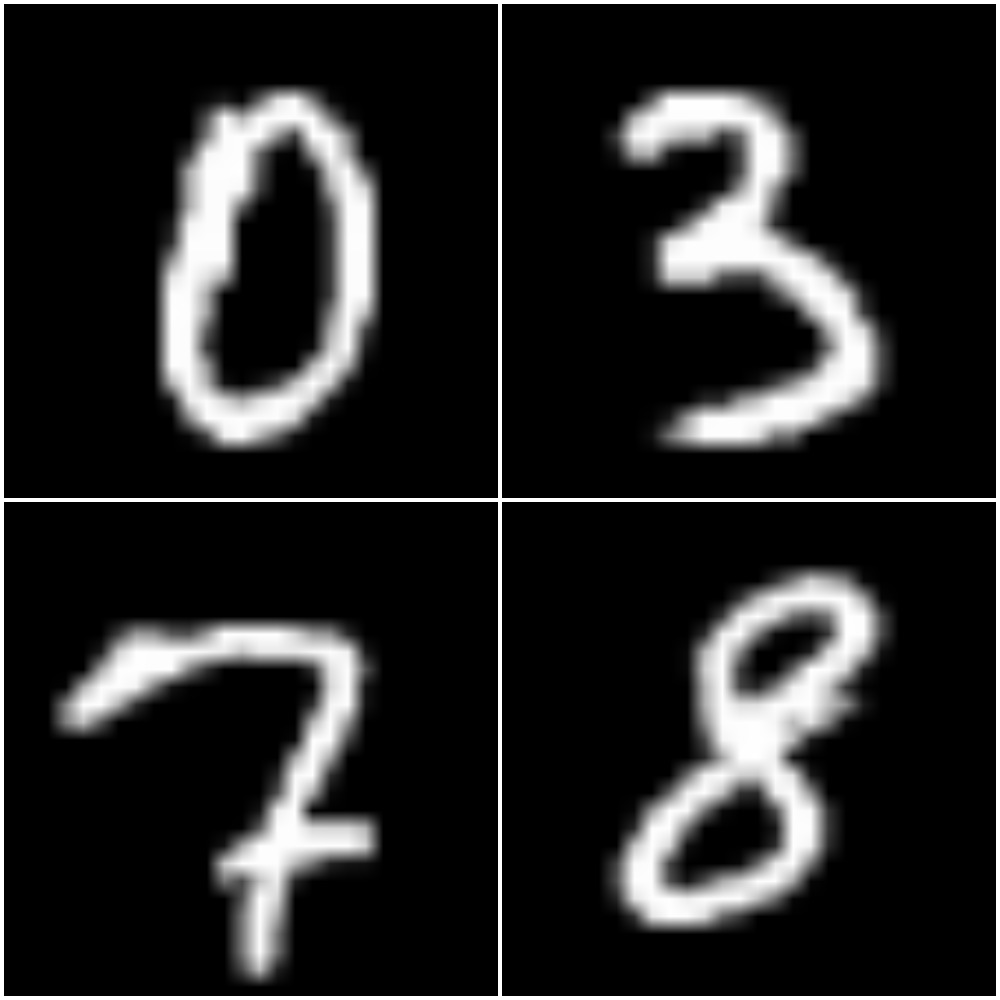
\includegraphics[width=4cm, height=4cm]{mnist_sample}
	\centering
	\caption{Sample images from MNIST dataset\cite{mnist}}
	\label{fig:mnist}
\end{figure}

With classifying digits, we have $10$ different classes i.e., $\{0, 1, 2, 3, 4, 5, 6, 7, 8, 9\}$. Since this is a multi-class classification problem (there are more than $2$ classes), we will employ the one-vs-all classification technique. In this technique, we construct $10$ different hyperplanes - each hyperplane distinguishes the input image between one class and the rest. For example, one such hyperplane would classify the input image as either $0$, or not. Another hyperplane would classify the input image as either $9$, or not. Thus, we end up with $10$ different hyperplanes. Note that we need $10$, and not $9$, hyperplanes to take into consideration the possibility that the image we are classifying might not be any of the $10$ digits. With this method, we run into the possibility of the same image being assigned to two different classes. When that happens, we will choose the hyperplane that gives a higher output value for the image.

Let us introduce some old notation to our new data. Let the number of images we have be $m$. Our $\vec{X}\in\mathbb{R}^{m}$, here, becomes a vector of all the images from the dataset. Let us denote each element of $\vec{X}$ as $\vec{x_i}$, which is, in turn, a single image from the dataset that is unrolled into a one dimensional vector. Let the length of the unrolled vectore be $n$. Therefore, $\vec{x_i}\in\mathbb{R}^{n}$. Each pixel value of the image becomes a feature in our feature space. Since we are working with grayscale images, we do not have to worry about RGB channels. Hence, it might make sense to think of $X$ as a matrix, $X\in\mathbb{R}^{m \times n}$.

Our ${y_i}$ associated with each of the $\vec{x_i}$ depends on the hyperplane we are constructing. Assume we are constructing the $k^{th}$ hyperplane i.e., the hyperplane that classifies the image as either digit $k$, or not digit $k$. Let us define the normal to this hyperplane as $\vec{w}^{(k)}$. Since our $y_i$ depends on the value $k$, let us re-define our notation as $y^{(k)}_i$, where
\begin{equation}
    y^{(k)}_i= 
\begin{cases}
 1,& \text{if } x_i \text{ represents } k\\
-1,              & \text{otherwise}
\end{cases}
\end{equation}

With this, we can now train the support vector machine and obtain our $10$ hyperplanes. As discussed previously, for predicting the digit on an image, we can use the modified equation
\begin{equation}
	f^{(k)}(x_i) = \vec{w}^{(k)}\cdot\vec{x_i} + b
\end{equation}
If $f^{(k)}(x_i) \geq 0$, then $\vec{x_i}$ represents $k$, and it does not represent $k$ otherwise. If, using this method, we find that $\vec{x_i}$ represents multiple $k_j$, then we choose a $k_a$ such that
\begin{equation}
	f^{(k_a)}(x_i) = \max_{j} f^{(k_j)}(x_i)
\end{equation}

To make computation simpler, we will set the intercept as the origin:
\begin{equation}
b = 0
\end{equation}